% ---------------------------------------------------------------------------
% DRAFT v2: organized around the current application (Hybrid Mute and Boost) with the journal history as development path. Every experimental claim in this file is traceable
% to a repository artifact listed in EVIDENCE_AUDIT.md. Items that need author
% confirmation are marked with \todo{...} and collected in RECONSTRUCTION.md.
% Compile: pdflatex main.tex (twice). No BibTeX run is needed (inline bibliography).
% ---------------------------------------------------------------------------
\documentclass[conference]{IEEEtran}
\IEEEoverridecommandlockouts
\usepackage[T1]{fontenc}
\usepackage{cite}
\usepackage{amsmath,amssymb}
\usepackage{graphicx}
\usepackage{booktabs}
\usepackage{xcolor}
\usepackage{tikz}
\usetikzlibrary{positioning,arrows.meta,fit}

\newcommand{\code}[1]{\texttt{\detokenize{#1}}}
\newcommand{\todo}[1]{\textcolor{red}{[TODO: #1]}}
\newcommand{\pp}{\,\mathrm{pp}}

\begin{document}

\title{Transient Activation Steering with a Pretrained Sparse Autoencoder for Suppressed Factual Completions in GPT-2 Small}

\author{\IEEEauthorblockN{Adithyan R S, Alona Biju, Alvin Binu, and Darsan M}
\IEEEauthorblockA{Department of Computer Science and Engineering (Artificial Intelligence)\\
Mar Baselios College of Engineering and Technology (Autonomous)\\
Thiruvananthapuram, Kerala, India\\
Guide: Ms.\ Poorna B R \todo{add author email addresses (Darsan M's institutional ID was not available)}}}

\maketitle


\begin{abstract}
A language model can give a correct completion non-trivial probability and still rank it below competing tokens. We describe FeatureScalpel, a system that corrects such suppressed completions at inference time, without changing weights, by scaling features of a pretrained sparse autoencoder (SAE) in the residual stream of GPT-2 small. The current system ranks candidate features by their measured causal effect, filters them one at a time, and applies a joint delta patch that mutes features driving the top competing token and boosts features supporting the target. It grows the edit one feature at a time, keeps the best step, and re-ranks candidates when a pool is used up. We trace how the system developed from single-feature ablation (1 and 3 of 22 suppressed facts corrected by the first two versions) using the project's research journal, and we evaluate the current pipeline. Drawing candidate features from all prompt positions instead of the last token reached rank 1 on 10 of 13 comparable prompts versus 4 of 13. The per-feature safety filter mattered: removing it lowered the number of prompts reaching rank 1 from 29 to 19 of 45, while relaxing it (tolerance or reduced strength) added at most one prompt across two studies. All results are for one model, one SAE release, mostly one layer, and prompts chosen by the authors. No comparison with other steering or model-editing methods has been performed.
\end{abstract}

\begin{IEEEkeywords}
sparse autoencoders, mechanistic interpretability, activation steering, factual recall, GPT-2
\end{IEEEkeywords}

\section{Introduction}
A language model can assign non-trivial probability to a correct completion and still rank it below other tokens. We call such a completion \emph{suppressed}. Repairing it with a weight edit changes the model for every later prompt~\cite{meng2022rome}. This paper studies a transient alternative: change the residual stream during one forward pass and discard the change afterwards. The direction of the change comes from a pretrained sparse autoencoder (SAE), so that concept-like components can be scaled down or up while the rest of the activation is left as it was.

The system, whose repository is named FeatureScalpel, is a research application. Its working version is the \emph{Hybrid Mute and Boost} workflow of \code{experiment_app.py}, with a headless twin used for batch studies. This paper describes that version (Section~\ref{sec:method}), records how it developed from earlier versions using the project's research journal (Section~\ref{sec:history}), and reports the experiments that were run on it (Section~\ref{sec:results}). Earlier versions and side experiments are treated as development history: they explain design decisions, but they are not part of what the system does today and they are not evaluated as competing methods.

This is not a comparison against other methods. No experiment in the repository compares the approach with weight editing, steering vectors, prompting, or any other baseline (Section~\ref{sec:future}). Each result is stated with the number of prompts it rests on, and Section~\ref{sec:limits} lists what the numbers do not show.

\section{Background and Related Work}
\subsection{Superposition and sparse autoencoders}
Elhage et al.\ describe a toy setting in which neurons respond to several unrelated inputs because a network stores more sparse features than it has neurons, a state they call superposition~\cite{elhage2022superposition}. Sparse autoencoders have been proposed as a way to recover the underlying directions. Bricken et al.\ train an SAE on the MLP activations of a one-layer transformer, using a linear encoder with a ReLU, a linear decoder, and a reconstruction loss with an L1 sparsity penalty, and report that in their human rating of feature descriptions the learned features were substantially more interpretable than neurons (median rubric score 12 versus 0)~\cite{bricken2023towards}. They also report that replacing the MLP output with the SAE output recovers 79\% of the log-likelihood loss reduction that the MLP provides for their main run~\cite{bricken2023towards}, so an SAE reconstruction is not exact. Cunningham et al.\ train SAEs on activations of a language model and report features that are more interpretable and more monosemantic than those found by alternative decompositions, as measured by automated methods, and that these features can localize causally responsible components on the indirect object identification task~\cite{cunningham2023sparse}.

This project uses a pretrained SAE rather than training one. The release is \code{gpt2-small-res-jb}, which provides one SAE for the residual stream input of each of the 12 blocks of GPT-2 small~\cite{bloom2024gpt2saes}. We loaded it through SAELens~\cite{bloom2024saelens} onto a GPT-2 small model~\cite{radford2019gpt2} run in TransformerLens~\cite{nanda2022transformerlens}.

\subsection{Steering with SAE features}
Wu et al.\ introduce AxBench, a benchmark of steering and concept detection on Gemma-2-2B and 9B, and report that, for steering, prompting outperforms all methods they test, followed by finetuning, and that SAEs are not competitive in their evaluation~\cite{wu2025axbench}. Our setting differs in model (GPT-2 small), task (raising the rank of one factual completion), and evaluation. We do not repeat their comparison, and nothing in this paper bears on their finding.

\subsection{Model editing}
Meng et al.\ locate factual recall in middle-layer feed-forward modules and introduce Rank-One Model Editing, which changes feed-forward weights to update a fact, together with a counterfactual dataset~\cite{meng2022rome}. The facts used in our development experiments were taken from the ROME \code{known_1000} data as recorded in \code{src/fact_bank.py}. The edits studied here do not change weights. We did not run ROME or any other editing method.


\section{Problem Formulation}
\label{sec:problem}
Let $x$ be a prompt, $p(v\mid x)$ the model's next-token distribution at the last position, and $t$ a target token. The rank of the target is $r(t)=1+\lvert\{v : p(v\mid x)>p(t\mid x)\}\rvert$. Tokens ranked above $t$ are competitors, and the top-1 token is the blocker. A fact is called \emph{already correct} if $r(t)=1$, \emph{suppressed} if $r(t)>1$ and either $p(t\mid x)>0.01$ or $r(t)\le 50$, and \emph{absent} otherwise. This is the rule implemented in \code{classify_fact} in \code{src/evaluation.py}.

An intervention is a set of per-feature scale factors applied at one layer. We say it \emph{reaches rank 1} if $r(t)=1$ under the edited forward pass. We also report the rank and probability of the target, the number of features edited, and a collateral measure defined in Section~\ref{sec:metrics}. The studies in Sections~\ref{sec:candsrc} and~\ref{sec:filter} use prompts whose target starts at rank 2 or worse, and do not apply the suppressed/absent split above, so some of their prompts would be classified as absent by that rule.

\section{The Current System}
\label{sec:method}
This section describes the pipeline as implemented in the Hybrid Mute and Boost tab of \code{experiment_app.py} and in its headless port \code{src/hybrid_runner.py}, which the batch studies use. The tab's defaults are mute strength 0.3, boost strength 0.5, at most 30 candidates, candidates drawn from all prompt positions, the safety filter on, and pool refill on when the cumulative sweep is enabled (the cumulative sweep itself is off by default). The studies of Section~\ref{sec:results} use other settings, stated with each study.

\subsection{Residual-stream edit through SAE features}
The SAE loaded for layer $L$ has a standard architecture with input width $d=768$, $m=24{,}576$ features, a ReLU, and the decoder bias subtracted from the input before encoding (the setting \code{apply_b_dec_to_input=True}). For a residual-stream activation $x$,
\begin{align}
f(x) &= \mathrm{ReLU}\!\big(W_e^{\top}(x-b_d)+b_e\big),\\
\hat{x}(f) &= W_d^{\top} f + b_d,
\end{align}
with $W_e\in\mathbb{R}^{d\times m}$ and $W_d\in\mathbb{R}^{m\times d}$. These are the encode and decode operations of the SAELens implementation used by the code.

An edit assigns a scale $s_i$ to each selected feature $i$ and forms $f'_i=s_i f_i$. The edited activation is the original activation plus the change in the decoded reconstruction,
\begin{equation}
x' = x + \hat{x}(f') - \hat{x}(f) = x + \sum_i (s_i-1)\, f_i\, w_i,
\end{equation}
where $w_i$ is row $i$ of $W_d$. Because the reconstruction error $x-\hat{x}(f)$ is not modified, the edit does not inject that error into the model, and $x'=x$ when all $s_i=1$. Muting a feature at strength $\mu\in[0,1]$ uses $s_i=1-\mu$ (so $\mu=1$ is full ablation), and boosting at strength $\beta\ge 0$ uses $s_i=1+\beta$. The hook is placed at \code{blocks.L.hook_resid_pre}, scales the chosen features at every token position, and the probabilities are read at the last position after the remaining blocks run. The hooks are removed after each forward pass, so nothing persists. Mute and boost edits in one intervention are applied in a single encode and decode from the same original activation. Section~\ref{sec:history} records the earlier chained implementation that the joint hook replaced.

\subsection{Candidate features}
\label{sec:candidates}
Candidates are features with positive activation. In \emph{last-token} mode they are the features active at the final prompt token. In \emph{all-positions} mode they are the features active at any non-BOS position, each scored by its maximum activation over those positions. A top-$N$ cut by activation is applied first, and $N$ is capped by the number of unapplied active features. Each candidate is then evaluated by fully ablating it alone ($s_i=0$) and recording the change $\Delta_i(v)=p_{\mathrm{abl}(i)}(v\mid x)-p(v\mid x)$ for a token $v$. Mute candidates are ordered by $\Delta_i(c)$ for the blocker $c$, most negative first. Boost candidates are ordered by $\Delta_i(t)$ for the target, most negative first, so they are the features whose removal hurts the target most.

\subsection{Safety filter}
\label{sec:safety}
The strict filter, which is the one the application applies (with an on/off switch), tests each candidate alone at the configured strength. A mute candidate is safe if the target's rank does not get worse and its probability does not fall by more than $10^{-6}$ (absolute); a boost candidate is tested the same way with its own strength. A separate combination check applies a whole set of edits together and reports \emph{new blockers}: tokens ranked below the target in the clean model that rise above it. Two relaxed variants of the per-feature rule exist only in the batch harness and were implemented for the study in Section~\ref{sec:filter}. In the \emph{tolerance} variant a candidate is also accepted if its probability drop is within $\max(10^{-6},\tau\,p(t\mid x))$ of the current target probability, with $\tau=0.05$. In the \emph{graded} variant a candidate that fails at full strength is retried at a fraction $\alpha$ of the configured strength. The first $\alpha$ is $0.95\,\theta/\lvert\Delta\rvert$, where $\theta$ is the same budget and $\Delta$ is the measured drop, and the retry is halved up to four times, giving up below $\alpha=0.05$. Accepted features that the strict rule would have rejected are used either after the strictly safe ones or in their natural order.

\subsection{Hybrid sweep and pool refill}
\label{sec:sweep}
The mute and boost pools are the safe candidates, ordered as above. (The application also offers user-specified batch-size lists instead of the cumulative sweep; the studies here use the cumulative sweep.) A feature that is safe on both sides is assigned to one side, chosen by which side raises the target probability more when the filter is on. The cumulative sweep evaluates step $k$ with the first $\min(k,M)$ mutes and $\min(k,B)$ boosts in one forward pass, where $M$ and $B$ are the pool sizes, and stops when the target reaches rank 1. The best step is the one with the lowest target rank, ties broken by higher probability, and this best step, not the last one, is reported. In \emph{pool refill}, when a pool is exhausted and the target is not yet rank 1, all applied features are kept, a forward pass with them applied gives a new baseline, the blocker becomes the top-1 token of that edited model, and candidates are re-ranked and re-filtered against it, including ones rejected earlier. A run ends at rank 1, when no unapplied active feature remains, when a round yields no safe candidate, or at an optional step limit.

\subsection{Batched evaluation}
\label{sec:batch}
Ranking and safety testing need one edited forward pass per candidate. The batched implementation repeats the prompt along the batch dimension, applies a different single-feature scale in each row through one hook, and computes the target rank on the device as the number of vocabulary entries with higher probability plus one. Batches are chunked at 32 rows. With the sequential path as reference, the journals report identical orderings and safety decisions (Section~\ref{sec:compute}).


\section{System Architecture}
\label{sec:arch}
Figure~\ref{fig:arch} shows the components that exist in the code. The clean pass caches the residual stream at the hook point for all positions. The candidate stages, the safety filter, and the sweep are in \code{src/editing.py}, \code{src/batched_eval.py}, and the hybrid runner. The hooks are in \code{src/hooks.py}. A batch runner executes lists of prompts under several filter settings and produces the paired comparisons in Section~\ref{sec:filter}. The application also contains an optional language-model explanation feature, monosemanticity diagnostics, a session-history recorder, and a timing comparison of the sequential and batched paths; none of these is evaluated here beyond the timing comparison of Section~\ref{sec:compute}.

\begin{figure}[t]
\centering
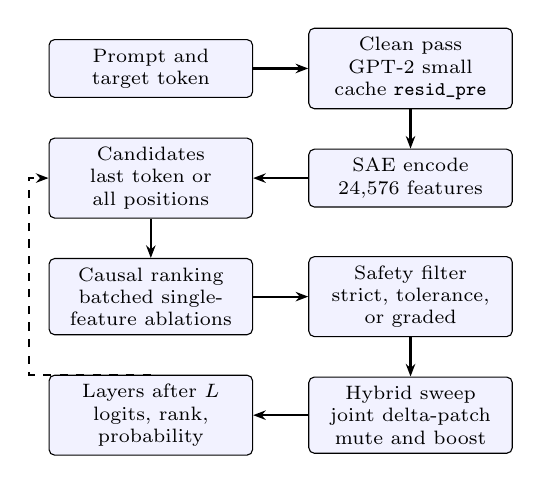
\begin{tikzpicture}[
  node distance=5mm and 7mm,
  box/.style={draw, rounded corners=2pt, align=center, font=\scriptsize, minimum height=7mm, text width=2.35cm, fill=blue!5},
  arr/.style={-{Stealth[length=1.6mm]}, thick}]
  \node[box] (in) {Prompt and\\target token};
  \node[box, right=of in] (clean) {Clean pass\\GPT-2 small\\cache \code{resid_pre}};
  \node[box, below=of clean] (sae) {SAE encode\\24,576 features};
  \node[box, left=of sae] (cand) {Candidates\\last token or\\all positions};
  \node[box, below=of cand] (rank) {Causal ranking\\batched single-\\feature ablations};
  \node[box, right=of rank] (safe) {Safety filter\\strict, tolerance,\\or graded};
  \node[box, below=of safe] (sweep) {Hybrid sweep\\joint delta-patch\\mute and boost};
  \node[box, left=of sweep] (out) {Layers after $L$\\logits, rank,\\probability};
  \draw[arr] (in) -- (clean);
  \draw[arr] (clean) -- (sae);
  \draw[arr] (sae) -- (cand);
  \draw[arr] (cand) -- (rank);
  \draw[arr] (rank) -- (safe);
  \draw[arr] (safe) -- (sweep);
  \draw[arr] (sweep) -- (out);
  \draw[arr, dashed] (out.north) -- ++(0,0.0) |- ++(-1.55,0.0) |- (cand.west);
\end{tikzpicture}
\caption{Components of the implemented pipeline. The dashed arrow marks pool refill: after a round, the applied features are kept and candidates are re-ranked against the edited model. Only components present in the code are shown.}
\label{fig:arch}
\end{figure}


\section{Development Path}
\label{sec:history}
The research journal (entries 1 to 20) and the project timeline record how the system reached its current form. Table~\ref{tab:history} compares each recorded stage with what the application does today. The right-hand column was checked against \code{experiment_app.py} and the source in \code{src/}. We use the journal for what was tried and what was recorded; where a journal statement has no stored output, we say so in the text or leave it out.

\begin{table*}[t]
\caption{Development stages recorded in the journal and their status in the current application. Dates are those of the journal entries (2026).}
\label{tab:history}
\centering\footnotesize
\begin{tabular}{@{}p{1.6cm}p{5.0cm}p{5.0cm}p{4.4cm}@{}}
\toprule
Entries (date) & Change & Recorded outcome & In the current application\\
\midrule
1, 2 (Jul 10--19) & Causal feature selector: rank active features by the probability change under ablation; iteratively ablate the top feature supporting the target (strength 0.3, up to 5 rounds) & 1 of 22 suppressed facts corrected & The ranking by ablation effect is kept. Target-supporting features are no longer muted; they are the boost candidates\\
3 (Jul 20) & Ablate the top feature driving the current top-1 token instead & 3 of 22 corrected, all at clean rank 2 & Kept: these are the mute candidates\\
4 (Jul 22--24) & Hybrid mute and boost in one intervention; whole-combination safety check & MIT-prompt sweep (Table~\ref{tab:hybrid}) & Kept: this is the current workflow\\
4, 6--8 (Jul 24--25) & Weighted multi-competitor reduction and top-$K$ variants, explored on one prompt & Seven competitors mapped to two features; rank 8 to 6 at best & Not in the application; code remains in \code{src/editing.py} without a user interface\\
9--11 (Aug 4--6) & Audit of the pretrained SAE; layer benchmark; stage profiling & Layer 8 had the highest mean rank gain on 12 prompts (Section~\ref{sec:layers}) & Layer 8 is the default; the benchmark harness remains\\
12--15 (Aug 9--Sep 18) & Delta patch formalized; safety filter stops recomputing the clean baseline; candidate ranking and safety tests batched on the GPU & 186 to 6 model forward calls for one evaluation, same selected features (Section~\ref{sec:compute}) & Kept, on by default; the sequential path is a switch\\
16 (Sep 18) & Best-so-far tracking & Rank could fluctuate across sweep steps, and the last step could be worse than an earlier one & Kept\\
17 (Sep 18) & Cumulative sweep: add one mute and one boost feature per step & Restores the original incremental search & Kept as an option\\
18 (Sep 18) & One joint hook replaces two chained hooks; explanation model migrated & Rank 66 (chained) versus 59 (joint) on one case & Kept; explanations are optional\\
19 (Sep 24) & Pool refill: keep applied features, re-rank and re-filter against the edited model & A run on ``black'' stopped at rank 5 after 24 features per side; 67 active features at the last token for another prompt & Kept, on by default\\
20 (Sep 25--26) & Candidate source option (last token or all positions); batch runner & 10 of 13 versus 4 of 13 reach rank 1 (Section~\ref{sec:candsrc}) & Kept; all positions is the default\\
Sep 26 (packs) & Safety-filter study: strict, none, tolerance, graded & Strict kept; relaxed rules add at most one prompt (Section~\ref{sec:filter}) & Strict only in the application; relaxed rules only in the batch harness\\
\bottomrule
\end{tabular}
\end{table*}

Three earlier ideas are no longer part of the system. Muting features that support the target lowered the target's own probability, so target-supporting features are boosted instead. Chained mute and boost hooks were replaced by one joint hook. Weighted multi-competitor reduction was replaced as the working method by the hybrid sweep. The remainder of this section gives the recorded numbers behind the first two stages and the one-prompt case that motivated best-so-far tracking.

\subsection{First versions: iterative ablation}
\label{sec:stage1}
The first evaluation ran iterative single-feature ablation at strength 0.3 for up to five rounds on 22 suppressed facts, in two variants: ablating the top feature supporting the target (variant~A) and ablating the top feature driving the current top-1 token (variant~B). After a success, the same features were applied to 15 control prompts, and specificity is the fraction of controls whose top-1 token was unchanged. Variant~A corrected 1 of 22 facts and variant~B corrected 3 of 22 (Table~\ref{tab:stage1}). Specificity was 100\% for all four successes.

\begin{table}[t]
\caption{Iterative ablation on 22 suppressed facts (strength 0.3, at most 5 rounds).}
\label{tab:stage1}
\centering\footnotesize
\begin{tabular}{@{}lccl@{}}
\toprule
Variant & Successes & Rounds & Corrected facts (clean rank)\\
\midrule
A: target features & 1/22 & 3 & Francesco Castellacci (2)\\
B: competitor features & 3/22 & 1, 1, 1 & Castellacci, Giulio Romano, Coco Chanel (all 2)\\
\bottomrule
\end{tabular}
\end{table}

All four successes started at clean rank 2, and 9 of the 22 facts started at rank 2. The top-1 token was ``the'' in 8 of the 22 facts, and none of those 8 succeeded. The top-1 tokens for the three variant-B successes were ``Italy'', ``P'' and ``May''. A journal narrative attributes the single variant-A success to the Eiffel Tower prompt, but the result tables list Castellacci and the fact set contains no Eiffel Tower prompt; we report the table. A second experiment on the same 22 facts ran single-shot joint ablation of the top competitor features against the clean top-1 token for strengths 0.3, 0.5, and 0.7 and batch sizes 1, 3, 5, and 10. It reached rank 1 on 2 to 4 of the 22 facts per setting, on 5 distinct facts in total, all with clean rank 2 (from \code{outputs/stage_1/grid_sweep_results.csv}; there is no journal entry for this run). These runs show why single-feature ablation was not enough: facts that start below rank 2 were not corrected by them.

\subsection{One prompt: competitor features and the hybrid sweep}
\label{sec:cambridge}
The prompt ``The location of Massachusetts Institute of Technology is in'' with target `` Cambridge'' has clean rank 8 and probability 1.15\%. Seven tokens rank above it: `` the'' (17.95\%), `` a'' (10.53\%), `` question'' (7.51\%), `` jeopardy'' (2.71\%), `` an'' (2.63\%), `` danger'' (1.76\%), and `` doubt'' (1.21\%). The journals record that the top-ranked driving feature of each competitor was feature 313 for `` the'', `` a'', and `` an'', and feature 21169 for the other four. The weighted-reduction experiments on this prompt (muting these features in proportion to competitor probability) left the target at rank 8 (1.29\% with the maximum rule, 1.39\% with the sum rule), and spreading the mute over each competitor's top three features gave rank 6. These experiments were one prompt with one run per setting, and they were not continued. They are recorded here because they showed that a few features are shared by many competitors, which is one reason the current sweep selects features by measured effect rather than by a fixed per-competitor rule.

A sweep of the hybrid intervention on the same prompt (mute and boost strength 1.0) gave Table~\ref{tab:hybrid}. With the safety filter applied, the best combinations reached rank 2. With the unfiltered candidates, three mutes and three boosts reached rank 1 (7.33\% against 6.98\% and 6.78\%), and adding a fourth boost feature (24181) returned the target to rank 2, because the probability of `` the'' rose while that of `` Cambridge'' fell. Running the same four-boost edit alone on a clean model gave the identical result (6.7357\%, rank 2), which rules out leftover hook state. The rank can also improve while the target's probability falls (4.28\% to 3.80\% while the rank went from 4 to 3). Adding features that were individually judged safe therefore does not guarantee a monotone improvement, and this is why the sweep reports its best step (Entry 16).

\begin{table}[t]
\caption{Hybrid sweep on the MIT prompt (strength 1.0 for both). Safe = candidates passing the per-feature filter; raw = unfiltered top candidates.}
\label{tab:hybrid}
\centering\footnotesize
\begin{tabular}{@{}llcc@{}}
\toprule
Candidates & Mutes / boosts & Rank & Target prob.\ (\%)\\
\midrule
safe & 1 / 1 & 5 & 2.20\\
safe & 1 / 3 & 3 & 4.81\\
safe & 2 / 3 & 2 & 7.81\\
safe & 3 / 3 & 2 & 8.59\\
raw & 3 / 3 & 1 & 7.33\\
raw & 3 / 4 & 2 & 6.74\\
\bottomrule
\end{tabular}
\end{table}

\section{Experimental Methodology}
\label{sec:methodology}
\subsection{Model, SAE, and hardware}
All experiments use GPT-2 small (117M parameters, 12 layers, $d_{\text{model}}=768$~\cite{radford2019gpt2}) loaded with TransformerLens defaults, and the pretrained SAE for \code{blocks.L.hook_resid_pre}, mainly $L=8$. The SAE metadata reports training on OpenWebText with context size 128 and BOS prepended. The system began as a CPU-only implementation and moved to GPU execution with batched candidate evaluation (Section~\ref{sec:compute}). The two safety-filter studies of Section~\ref{sec:filter} ran on a consumer GPU (GTX 1660 Ti, PyTorch 2.6.0, CUDA 12.4). Absolute timings depend on the hardware and are used here only to compare implementations.

\subsection{Prompts}
\label{sec:prompts}
\emph{Fact bank.} \code{src/fact_bank.py} holds 45 (prompt, target) pairs from ROME \code{known_1000}, all with single-token targets. The rule of Section~\ref{sec:problem} labeled 15 as already correct, 8 as absent, and 22 as suppressed. The 22 suppressed facts form the evaluation set of the first versions (Section~\ref{sec:stage1}), and the 15 already-correct facts serve as control prompts.

\emph{Layer benchmark set.} \code{benchmark_test_prompts.json} lists 22 prompts. The 21-prompt run analyzed in Section~\ref{sec:layers} used all of them except one (``Eavan Boland was born in). In that run 9 prompts had the target at rank 1 in the clean model and 12 did not, with clean ranks 2 (six prompts), 8 (two), 10, 16, 45, and 84.

\emph{Candidate-source prompts.} A set of 17 prompts assembled by the authors (factual and commonsense completions): 14 with the target below rank 1 and 3 with the target already at rank 1 (Section~\ref{sec:candsrc}).

\emph{Informal checks.} During development the pipeline was also tried by hand on other prompts, including ad hoc ones, and the authors observed it working there as well. Those runs were not recorded and are not evidence in this paper.

\emph{Safety-filter prompt set.} \code{data/safety_filter_prompts_full.json} holds 211 prompts whose target is a single GPT-2 token with a leading space. They come from the 17 prompts above, both 22-prompt ROME files in the repository, templated country facts (capital, language, currency), and hand-written factual and commonsense prompts. Baseline ranks were measured with the clean model. Of these, 131 have target rank 2 to 1000, 4 have a rank above 1000 (not used), and 76 have rank 1. The pilot study used 45 of the 131 (a seeded stratified sample of 10, 10, 10, 10, and 5 prompts from the rank bins 2 to 3, 4 to 10, 11 to 50, 51 to 300, and 301 to 1000), plus 5 rank-1 controls. The full last-token study used all 131 plus 25 sampled controls. The prompts are not a random sample, and many share templates, so they are not independent draws.

\subsection{Metrics and protocol}
\label{sec:metrics}
The main measure is whether the target reaches rank 1 in the sweep, together with the final rank, the number of features edited at the best step, the number of sweep steps, and model compute time. \emph{Collateral change} is the mean KL divergence $D_{\mathrm{KL}}(p_{\text{clean}}\,\|\,p_{\text{edited}})$ at the last position over 20 fixed neutral prompts, with the best step's per-feature scales applied, and the fraction of those prompts whose top-1 token changes. A feature that is inactive on a neutral prompt cannot change it, so this measures interference only where the edited features fire. It is not the specificity metric of earlier experiments (Section~\ref{sec:stage1}) and not a CounterFact-style score. In the safety-filter studies the per-step new-blocker report was switched off for speed, and the rank at each step was computed from the same forward pass that produced the top-5 table. Each prompt and condition was run once. Runs were reproducible: re-running the 34-run batch of Section~\ref{sec:candsrc} from the application and from a command-line script gave identical feature lists, steps, and probabilities in every run.

For the paired comparisons, one arm is better than another on a prompt if it reaches rank 1 when the other does not, or, when both agree on that, if its final rank is lower. We report exact two-sided sign tests on prompts that differ and exact McNemar tests on the change in reaching rank 1. No correction was made for multiple comparisons.


\section{Experimental Results}
\label{sec:results}
The studies below evaluate the pipeline of Section~\ref{sec:method}. The layer sweep was run with the benchmark harness, which used fixed-size steps and last-token candidates, without pool refill. The two later studies used the batch runner, which reproduces the application's workflow.

\subsection{Depth of the intervention}
\label{sec:layers}
On the MIT prompt, a hybrid intervention (mute 0.3, boost 0.5, three features each, safety filter on) at layers 2, 5, 8, and 10 raised the target from rank 8 to 7, 5, 3, and 5, with probability gains of 0.07, 0.78, 2.38, and 0.81 percentage points (Fig.~\ref{fig:mitlayers}; artifact \code{layer_benchmark_20260909_143704_240449.json}). The journal entry and its plots give 0.79, 2.37, and 0.82 for three of these, which differ from the stored file by at most 0.01 points. The top-1 token stayed `` the'' in all four. This is one prompt.

\begin{figure}[t]
\centering
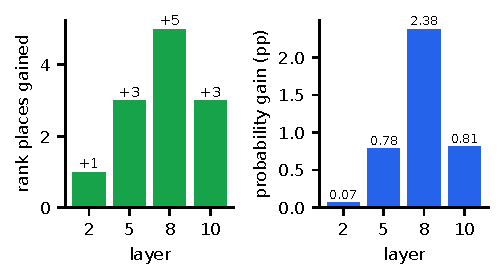
\includegraphics[width=\columnwidth]{figures/fig_mit_layers.pdf}
\caption{Rank places gained (left) and target probability gain in percentage points (right) at layers 2, 5, 8, and 10 on the MIT prompt. One prompt, one run per layer, drawn from the stored benchmark file.}
\label{fig:mitlayers}
\end{figure}

A larger run covered 21 prompts and all 12 layers (mute 0.6, boost 0.7, three features each, safety filter on, last-token candidates). We summarize the 12 prompts whose target was not already at rank 1 (Fig.~\ref{fig:layer12}, Table~\ref{tab:layers}). The mean rank gain was highest at layer 8 (7.33), close to layers 7 (7.08), 6 (6.50), and 9 (6.33), and at most 2.7 at layers 0 to 3, 5, and 11. Layer 8 improved the rank on 9 of the 12 prompts and reached rank 1 on 3. Layer 8 is therefore not clearly separated from its neighbors on this sample, and the parameters and candidate mode differ from those of the later studies.

\begin{figure}[t]
\centering
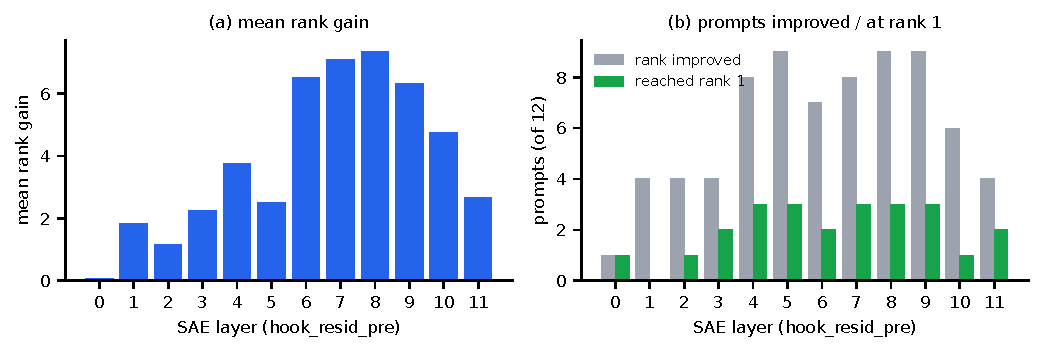
\includegraphics[width=\columnwidth]{figures/fig_layer12.pdf}
\caption{Twelve prompts with target below rank 1, all 12 layers (mute 0.6, boost 0.7, three features each). (a) Mean rank gain. (b) Prompts whose rank improved and prompts that reached rank 1.}
\label{fig:layer12}
\end{figure}

\begin{table}[t]
\caption{Layer sweep on 12 prompts with clean rank above 1 (from \code{tools/summarize_layer_benchmark.py}).}
\label{tab:layers}
\centering\footnotesize
\begin{tabular}{@{}cccccc@{}}
\toprule
Layer & Rank 1 & Improved & Worse & Mean gain & Median final rank\\
\midrule
0 & 1 & 1 & 0 & 0.08 & 5.0\\
1 & 0 & 4 & 1 & 1.83 & 4.5\\
2 & 1 & 4 & 1 & 1.17 & 3.0\\
3 & 2 & 4 & 2 & 2.25 & 3.0\\
4 & 3 & 8 & 1 & 3.75 & 3.0\\
5 & 3 & 9 & 0 & 2.50 & 2.5\\
6 & 2 & 7 & 0 & 6.50 & 2.5\\
7 & 3 & 8 & 1 & 7.08 & 2.5\\
8 & 3 & 9 & 0 & 7.33 & 2.5\\
9 & 3 & 9 & 0 & 6.33 & 3.0\\
10 & 1 & 6 & 1 & 4.75 & 3.5\\
11 & 2 & 4 & 0 & 2.67 & 2.0\\
\bottomrule
\end{tabular}
\end{table}

\subsection{Where candidate features are drawn from}
\label{sec:candsrc}
Candidates from the last token only can be a small set. For ``The leading cause of death in men is'' at layer 8, 67 features were active at the last token and 303 across all positions, and a run with pool refill used all 67 of the former (rank 152 to 50 with a candidate limit of 10 per round, and rank 51 when all 67 were used). The journal notes that scaling cannot switch on an inactive feature, so the active set bounds any single-layer, single-position edit of this kind.

We compared the two candidate sources on 17 prompts with mute 0.6, boost 0.5, and Top-$N$ 120 at layer 8, with the safety filter on and pool refill on. Of the 17, three had the target already at rank 1 (no edit was made in either mode) and one had a two-token target whose last piece was scored, so it is excluded. Table~\ref{tab:candsrc} and Fig.~\ref{fig:candsrc} give the 13 comparable prompts. All-positions candidates reached rank 1 on 10 of 13 prompts and last-token candidates on 4 of 13. All-positions won on 9 prompts, the modes tied on 4 (both at rank 1), and last-token won on none, giving an exact two-sided sign test $p\approx0.004$ on the 9 prompts that differed. The final target probability was higher with all positions on 12 of 13 prompts and identical on one. The mean number of candidate features at round 0 was 281 for all positions and 56 for last token. All 9 last-token failures ended because no unapplied active feature remained. Where both modes reached rank 1, last-token used no more features than all-positions (last versus all: 2 and 2, 12 and 16, 2 and 2, 47 and 118). All-positions used on average 94 features against 42 and about twice the compute time (12.2 s against 5.4 s per run). Three prompts failed in both modes (Colosseum, the door prompt, and ``The doctor said that''), and all-positions still ended at a better rank on each.

\begin{figure}[t]
\centering
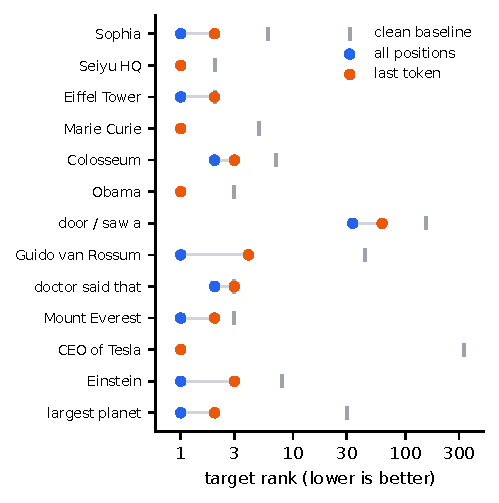
\includegraphics[width=0.85\columnwidth]{figures/fig_candidate_source.pdf}
\caption{Final target rank per prompt for the 13 comparable prompts (log scale). The tick marks the clean baseline rank.}
\label{fig:candsrc}
\end{figure}

\begin{table}[t]
\caption{Candidate source study. Final rank of the target (rank 1 = reached).}
\label{tab:candsrc}
\centering\footnotesize
\begin{tabular}{@{}lccc@{}}
\toprule
Prompt (target) & Clean & All positions & Last token\\
\midrule
This is Sophia, she is a (woman) & 6 & 1 & 2\\
Seiyu Group's headquarters are in (Tokyo) & 2 & 1 & 1\\
The Eiffel Tower is in the city of (Paris) & 2 & 1 & 2\\
Marie Curie won the Nobel Prize in (Physics) & 5 & 1 & 1\\
The Colosseum is located in (Rome) & 7 & 2 & 3\\
Barack Obama was born in (Hawaii) & 3 & 1 & 1\\
She opened the door and saw a (cat) & 152 & 34 & 62\\
Language created by Guido van Rossum is (Python) & 44 & 1 & 4\\
The doctor said that (she) & 3 & 2 & 3\\
Mount Everest is located in (Nepal) & 3 & 1 & 2\\
The CEO of Tesla is (Elon) & 335 & 1 & 1\\
Albert Einstein was born in (Germany) & 8 & 1 & 3\\
Largest planet in our solar system is (Jupiter) & 30 & 1 & 2\\
\bottomrule
\end{tabular}
\end{table}

\subsection{Safety-filter study}
\label{sec:filter}
The strict filter rejected roughly half the candidates at round 0, and we asked whether a less strict filter would help, because features that are rejected are not used. Five arms were run on identical prompts (Section~\ref{sec:safety}): the strict filter, no filter, tolerance 5\%, graded strength with tolerance 5\% (accepted features used after the strictly safe ones), and the same graded rule with accepted features in their natural order. Settings were mute 0.6, boost 0.5, Top-$N$ 120, pool refill on, and a limit of 250 sweep steps. Two studies were run: a pilot in all-positions mode on 45 prompts with target rank above 1 (5 controls were also run and excluded from the comparison), and a full study in last-token mode on 131 prompts. Neither study was run in the other mode. Table~\ref{tab:filter} and Fig.~\ref{fig:filter} give the results.

\begin{figure*}[t]
\centering
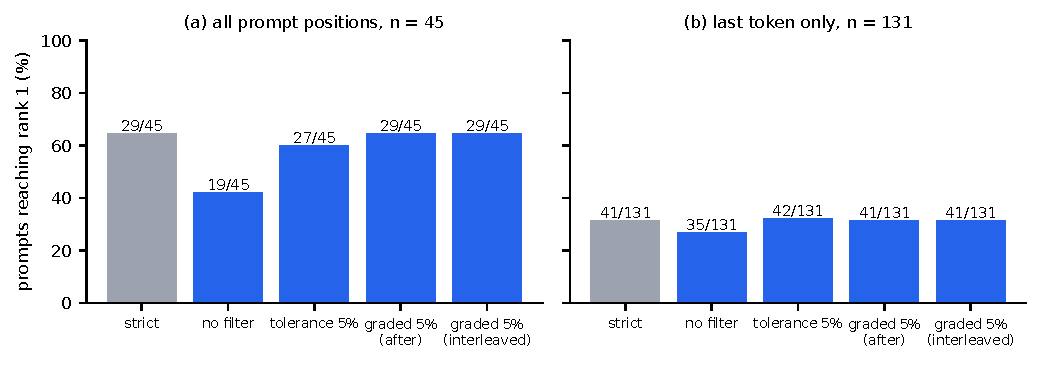
\includegraphics[width=0.85\textwidth]{figures/fig_filter.pdf}
\caption{Prompts reaching rank 1 under each safety-filter setting. (a) Pilot study, all prompt positions, 45 prompts. (b) Full study, last token only, 131 prompts. Counts are shown above the bars.}
\label{fig:filter}
\end{figure*}

\begin{table*}[t]
\caption{Safety-filter arms. Reached = prompts reaching rank 1. Features, steps, and time are means per run. KL is the mean collateral KL in nats. Better/Worse/Same compare each arm with the strict filter on the same prompts, followed by the number of prompts that newly reached or lost rank 1 and the exact p-values (sign test, McNemar; ``--'' where no prompt changed).}
\label{tab:filter}
\centering\footnotesize
\begin{tabular}{@{}llccccccccc@{}}
\toprule
Study & Arm & Reached & Features & Steps & Time (s) & KL & B/W/S & New/Lost & Sign $p$ & McNemar $p$\\
\midrule
Pilot, all, $n{=}45$ & strict & 29 & 120.4 & 68.0 & 6.5 & 0.0055 & (ref.) & & & \\
 & no filter & 19 & 132.5 & 89.6 & 7.1 & 0.0069 & 1/22/22 & 0/10 & $<0.001$ & 0.002\\
 & tolerance 5\% & 27 & 123.3 & 74.1 & 7.0 & 0.0056 & 2/3/40 & 0/2 & 1.0 & 0.50\\
 & graded, after & 29 & 125.9 & 70.8 & 6.6 & 0.0054 & 1/5/39 & 0/0 & 0.22 & --\\
 & graded, interleaved & 29 & 125.9 & 70.8 & 6.6 & 0.0054 & 1/5/39 & 0/0 & 0.22 & --\\
\midrule
Full, last, $n{=}131$ & strict & 41 & 43.2 & 26.6 & 2.5 & 0.0015 & (ref.) & & & \\
 & no filter & 35 & 41.6 & 25.8 & 2.0 & 0.0014 & 7/64/60 & 4/10 & $<0.001$ & 0.18\\
 & tolerance 5\% & 42 & 42.5 & 26.3 & 2.4 & 0.0015 & 2/9/120 & 1/0 & 0.065 & 1.0\\
 & graded, after & 41 & 42.7 & 26.3 & 2.7 & 0.0014 & 2/15/114 & 0/0 & 0.002 & --\\
 & graded, interleaved & 41 & 42.3 & 26.4 & 2.6 & 0.0014 & 3/13/115 & 0/0 & 0.021 & --\\
\bottomrule
\end{tabular}
\end{table*}

Removing the filter lowered the rate of reaching rank 1 from 29 to 19 of 45 prompts in the pilot, with 10 prompts lost and none gained, and it raised the collateral KL from 0.0055 to 0.0069. In the last-token study it worsened the final rank on 64 prompts and improved it on 7. Relaxing the filter added no prompt in the pilot and at most one in the full study. Graded strength gave a worse final rank on 13 to 15 of the 131 prompts in the last-token study, and its features and collateral change were close to those of the strict filter. Few rescued features were in the best result: on average 1.2 to 3.0 of about 125 features in the pilot and 0.4 to 1.1 of about 43 in the full study.

The strict filter's verdicts explain why relaxing it changed little (Table~\ref{tab:reasons}). At round 0, about half of the candidates (mute and boost sides pooled) were accepted, and most rejections were for harm (the target probability falling by more than $10^{-6}$), with 1.5 to 2.3\% failing only the rank rule and 13.9 to 15.0\% failing both. Only 157 of 5,400 candidate features (2.9\%) in the pilot and 195 of 7,691 (2.5\%) in the full study were unusable on both sides, because a feature rejected as a mute candidate is usually accepted as a boost candidate and the reverse. In the pilot, across all five arms, 83 of 250 runs ended because no unapplied active feature remained, 7 ended with no safe candidate in a round, 2 reached the step limit, 133 reached rank 1, and 25 were controls already at rank 1.

\begin{table}[t]
\caption{Strict-filter verdicts on round-0 candidates (mute and boost sides pooled).}
\label{tab:reasons}
\centering\footnotesize
\begin{tabular}{@{}lcc@{}}
\toprule
Verdict & Pilot (all) & Full (last)\\
\midrule
accepted & 5447 (50.4\%) & 7776 (50.6\%)\\
rejected, harm rule only & 3492 (32.3\%) & 5234 (34.0\%)\\
rejected, rank rule only & 245 (2.3\%) & 230 (1.5\%)\\
rejected, both rules & 1616 (15.0\%) & 2142 (13.9\%)\\
\bottomrule
\end{tabular}
\end{table}

\subsection{Cost of evaluating candidates}
\label{sec:compute}
In a profiled layer-8 run of the layer benchmark, feature selection (about 350 ms) and safety filtering (about 1,200 ms) accounted for most of the 1.88 s total, which is why we measured their cost. For one prompt and layer with 30 candidates on each side, a journal audit counted 186 model forward passes in the original implementation, 126 after the safety filter stopped recomputing the clean baseline, and 122 after clean-pass caching. Stacking the candidates into the batch dimension reduced the same evaluation to 6 forward calls (1 clean, 1 each for competitor ranking, target ranking, competitor safety, and target safety, and 1 final), while the number of edited sequences evaluated was unchanged. The audit reports identical selected features (mute 8459, 21169, 14430; boost 3076, 19288, 8239), identical probabilities to $10^{-9}$ in the caching step, zero ordering differences across six prompts for the batched ranking, and 60 of 60 identical safety decisions on the MIT prompt. Removing the redundant clean passes cut the safety stage from 3,863 ms to 1,953 ms and total time from 6.38 s to 4.39 s in that audit. In the application, the sequential and batched versions of one workflow took 12.16 s and 0.90 s, 11.55 s and 0.71 s, and 11.75 s and 0.58 s in three runs on one prompt, with the same result (rank 1, 13.42\%). The move from CPU to GPU was also measured: 3 prompts on 4 layers took 150.07 s on the GPU against 574.60 s on the CPU (3.83 times), with a peak of 1.48 GB of GPU memory. Together, GPU execution and batching are what made the large studies of Section~\ref{sec:results} feasible.


\section{Discussion}
The picture is consistent and limited. The first two versions of the system (single-feature ablation) corrected 1 and 3 of 22 suppressed facts, all of them at clean rank 2, which motivated combining muting of competitor features with boosting of target features in one joint edit. On the current pipeline, two results point to the supply of candidate features rather than to the selection rule. Drawing candidates from all positions increased the pool about fivefold and raised the number of prompts reaching rank 1 from 4 to 10 of 13, and every last-token failure ended by exhausting the active features. In the filter study, the strict filter removed few features for good (2.5 to 2.9\%), because it mostly sorts features into a mute side and a boost side. Relaxing it did not add prompts and removing it cost prompts, so the filter that the application already uses is the one supported by the data.

These results are consistent with the size of the active feature set being the main limit of a multiplicative edit at one layer, and they do not exclude other limits. In particular, scaling cannot activate a feature that is off, and we have not tested any mechanism that could. The metric matters: rank and probability can move in opposite directions (Section~\ref{sec:cambridge}), so we report rank-based outcomes and treat probability changes as secondary. The layer sweep suggests layer 8 is a reasonable choice, but on 12 prompts it is close to its neighbors, and the sweep used a different candidate mode and strengths from the later studies.

\section{Limitations}
\label{sec:limits}
\begin{itemize}
\item One model (GPT-2 small) and one SAE release, with layer 8 used in all later studies. Nothing here says the findings transfer to other models or layers.
\item The prompts were not drawn at random from a defined population: the pools were assembled from the ROME data, templated country facts, and hand-written prompts, and only the pilot subset was sampled at random (seeded, stratified by baseline rank). The prompts are few (22, 12, 13, 45, and 131 depending on the experiment), share templates, and are not independent samples. Statistical tests treat prompts as independent and are uncorrected for multiple comparisons.
\item Success means the target is top-1 on the next token for that prompt. Paraphrases, longer generations, and downstream behavior were not tested. Collateral change is measured only as KL on 20 neutral prompts, not with the specificity or neighborhood metrics of prior editing work.
\item No comparison with weight editing, steering vectors, prompting, or other SAE steering has been run, so nothing in this paper says how this approach ranks against them.
\item The development-stage results of Section~\ref{sec:history} were obtained with earlier versions of the system and on few prompts (one prompt in the case of the weighted-reduction experiments). They document the path taken, not the performance of the current system. Some development claims in the project's timeline (for example, a fix of Dublin and Melbourne prompts by the hybrid method) have no stored output and are not used.
\item Journal inconsistencies remain. The journals give 46 facts where the code and the category counts give 45. The stage-1 narrative names the Eiffel Tower prompt as the variant-A success while the tables name another fact. The layer benchmark's own \code{success} flag counts an improvement in rank or probability and is not used here. The PyTorch version in \code{requirements.txt} (2.13.0) differs from the one used for the studies (2.6.0 with CUDA 12.4).
\item The blocker is fixed within a round of pool refill, even if the top-1 token changes as features are applied.
\item The editing and safety code has no automated tests in the repository; the tests cover only the monosemanticity diagnostics. Equivalence between paths was checked with scripts recorded in the journals.
\item The scoring function keeps only the last token of a multi-token target, which affected one prompt in the candidate-source study and is excluded there. The safety-filter prompt set was restricted to single-token targets.
\end{itemize}

\section{Future Work}
\label{sec:future}
The following are planned or open and have \emph{not} been done. (1) Comparisons on the same prompts with weight editing~\cite{meng2022rome}, steering vectors, and prompting; the repository contains no code or results for these. (2) Testing other layers and combined layers with the same pipeline, and other models. (3) Re-selecting the blocker within a round when the top-1 token changes. (4) A larger side-effect evaluation than the 20-prompt KL. (5) Mechanisms that can use features that are inactive on the prompt. (6) A learned predictor of feature effects to replace per-candidate evaluation, and gradient-based attribution as a faster approximation of the ablation ranking. (7) Repeating the all-positions safety-filter study on the full 131 prompts (only the pilot subset has been run).

\section{Conclusion}
We implemented a transient residual-stream edit through SAE features of GPT-2 small and traced its development from single-feature ablation to a hybrid mute-and-boost sweep with a per-feature safety filter, best-step tracking, and pool refill. On the current pipeline, candidates drawn from all prompt positions reached rank 1 on more prompts than last-token candidates (10 of 13 against 4 of 13), and the per-feature safety filter was worth keeping, because removing it lost prompts while relaxing it gained at most one. These results are for one small model, mostly one layer, and prompts chosen by us, and they do not compare the method with any alternative.

\begin{thebibliography}{00}
\bibitem{bricken2023towards} T. Bricken \emph{et al.}, ``Towards Monosemanticity: Decomposing Language Models With Dictionary Learning,'' Transformer Circuits Thread, Anthropic, Oct. 2023. [Online]. Available: https://transformer-circuits.pub/2023/monosemantic-features/index.html
\bibitem{cunningham2023sparse} H. Cunningham, A. Ewart, L. Riggs, R. Huben, and L. Sharkey, ``Sparse Autoencoders Find Highly Interpretable Features in Language Models,'' arXiv:2309.08600, 2023.
\bibitem{elhage2022superposition} N. Elhage \emph{et al.}, ``Toy Models of Superposition,'' arXiv:2209.10652, 2022.
\bibitem{meng2022rome} K. Meng, D. Bau, A. Andonian, and Y. Belinkov, ``Locating and Editing Factual Associations in GPT,'' in \emph{Advances in Neural Information Processing Systems}, vol.~35, 2022.
\bibitem{wu2025axbench} Z. Wu, A. Arora, A. Geiger, Z. Wang, J. Huang, D. Jurafsky, C. D. Manning, and C. Potts, ``AxBench: Steering LLMs? Even Simple Baselines Outperform Sparse Autoencoders,'' arXiv:2501.17148, 2025.
\bibitem{radford2019gpt2} A. Radford, J. Wu, R. Child, D. Luan, D. Amodei, and I. Sutskever, ``Language Models are Unsupervised Multitask Learners,'' OpenAI, technical report, 2019. \todo{confirm year and preferred citation form}
\bibitem{nanda2022transformerlens} N. Nanda and J. Bloom, ``TransformerLens,'' 2022. [Online]. Available: https://github.com/TransformerLensOrg/TransformerLens
\bibitem{bloom2024saelens} J. Bloom, C. Tigges, A. Duong, and D. Chanin, ``SAELens,'' 2024. [Online]. Available: https://github.com/decoderesearch/SAELens
\bibitem{bloom2024gpt2saes} J. Bloom, ``Open Source Sparse Autoencoders for all Residual Stream Layers of GPT2-Small,'' LessWrong, Feb. 2, 2024. [Online]. Available: https://www.lesswrong.com/posts/f9EgfLSurAiqRJySD/open-source-sparse-autoencoders-for-all-residual-stream
\end{thebibliography}

\end{document}
